\section{方法选择}
\label{sec:budget-selection}

前三节给出了比较的尺子：误差口径、成本账和预算分配。还缺的是候选名单。一个方法能不能用，取决于目标分布和被积函数给了哪些可以计算的东西：能否计算分布函数的逆，能否逐点计算密度、只到一个常数因子还是完整归一化，能否对样本位置求导，是否知道某些辅助函数的精确期望。表~\ref{tab:budget-information}把前几章的方法按所需信息排列。

\begin{BookInlineTable}
  \centering
  \caption{可计算的信息与相应的方法}
  \label{tab:budget-information}
  \begin{tabular}{@{}p{44mm}p{62mm}@{}}
    \toprule
    可以计算的量 & 可用的方法 \\
    \midrule
    分位数函数 & 逆变换采样 \\
    混合成分或逐坐标条件分布 & 分步生成 \\
    有限包络常数下的密度比 & 拒绝采样 \\
    未归一化密度的比值 & MCMC，自归一化重要性采样 \\
    可采样且可计算密度的建议分布 & 重要性采样 \\
    期望已知的辅助函数 & 控制变量 \\
    精确的条件期望 & 条件期望降方差 \\
    层概率与层内条件抽样 & 分层采样 \\
    均匀输入下的生成映射 & 拉丁超立方，随机化准蒙特卡洛，对偶变量 \\
    被积函数对样本位置的导数 & 重参数化梯度 \\
    密度对参数的对数导数 & 得分函数梯度 \\
    \bottomrule
  \end{tabular}
\end{BookInlineTable}

名单只说明“可以用”，不说明“值得用”。一个方法可用而且理论上正确，并不意味着它在当前预算下比更朴素的方法有效。选择的依据始终是同一任务、同一误差口径下的总成本：先列出所有可用方案，再按第~\ref{sec:budget-costs}节的账估算每个方案的$\sigma^{2}c$和一次性开销，最后按预算决定。下面三小节分别对采样、方差控制和梯度估计做这件事。

\subsection{采样方法的选择}
\label{sec:budget-sampler-choice}

生成样本的方法大致按“需要的信息越多，结果越好”排列。直接生成（逆变换、分步生成）给出独立且精确服从目标的样本，每个样本成本固定；拒绝采样同样给出独立精确的样本，但每个输出平均要付出$M$个候选的成本；MCMC只需要未归一化密度的比值，代价是样本相关，而且要另行核验初值影响与探索范围。图~\ref{fig:budget-sampler-choice}把检查的顺序画成流程：从最强的信息问起，能用的第一个方法往往是成本最低的，但每个方法框右侧列出的量仍要逐项核对。

\begin{BookInlineFigure}
  \centering
  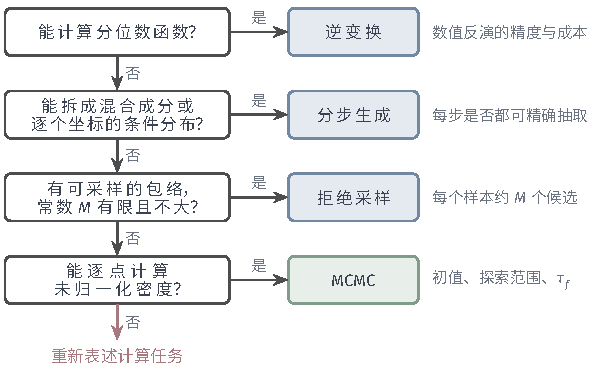
\includegraphics[width=101mm]{figures/07-probability/08-sampling-and-integration/tikz/budget-sampler-choice/figure.pdf}
  \caption{选择采样方法时依次检查的信息。左列从上到下要求的信息逐渐减少；每个方法框右侧是选定该方法后仍要比较的量：数值反演的精度、分步是否都能精确抽取、平均候选数$M$、链的初值影响与$\tau_{f}$。四项都不满足时（红色）需要改变计算任务的表述，例如换一个积分表示。}
  \label{fig:budget-sampler-choice}
\end{BookInlineFigure}

\paragraph{直接生成的数值精度}
分位数函数没有解析式时，逆变换要数值求解$F(x)=u$。用二分法在长度为$L$的区间上把$x$定位到容差$\eta$，需要约$\log_{2}(L/\eta)$次分布函数计算。容差带来一个确定性的偏差：输出不再精确服从$F$，而是服从相应的近似分布，第~\ref{chap:monte-carlo-integration-error}章说明这种偏差不随样本数减小。所以$\eta$要按最终的误差要求定：若$f$满足Lipschitz条件$\lvert f(x)-f(y)\rvert\le L_f\lvert x-y\rvert$，而数值反演把每个样本移动不超过$\eta$，则偏差不超过$L_f\eta$，取$L_f\eta$远小于$\varepsilon$即可，每个样本多付出的只是对数级的求值次数。

例如在长度$L=50$的区间上定位到$\eta=10^{-8}$，需要$\lceil\log_{2}(5\times10^{9})\rceil=33$次分布函数计算，比解析的逆变换贵几十倍，但仍可能比拒绝采样或MCMC便宜。分步生成要求每一步都能精确抽取；某一步只能近似时，整条生成链的偏差按同样方式核对。

\paragraph{拒绝采样的包络与尾部}
拒绝采样的成本由$M=\sup_{x}p(x)/q(x)$决定，而$M$有限要求包络在每个方向上的尾部不比目标轻。以$t_{3}$分布为目标，它的密度按$\lvert x\rvert^{-4}$衰减。用高斯包络$q_{1}=\mathcal{N}(0,2^{2})$时，比值
\[
  \frac{p(x)}{q_{1}(x)}\propto\Bigl(1+\frac{x^{2}}{3}\Bigr)^{-2}\mathrm{e}^{x^{2}/8}\to\infty,
\]
不存在有限的$M$；用Cauchy包络$q_{2}(x)=1/\bigl(\pi(1+x^{2})\bigr)$时比值有界，在$x=\pm1$处取最大值，网格计算得$M\approx1.30$。图~\ref{fig:budget-rejection-tails}画出这两种情形。

\begin{BookInlineFigure}
  \centering
  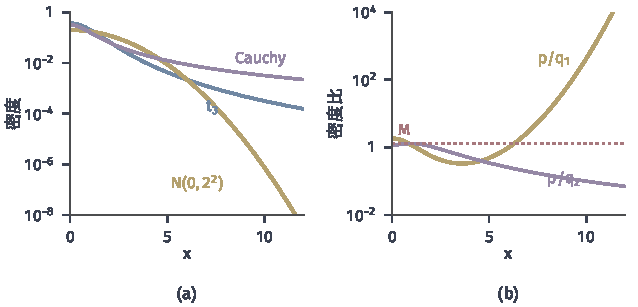
\includegraphics[width=108mm]{figures/07-probability/08-sampling-and-integration/matplotlib/budget-rejection-tails/figure.pdf}
  \caption{拒绝采样的包络必须覆盖目标的尾部。(a)~目标$t_{3}$（蓝）与两个包络的密度，对数纵轴：高斯$\mathcal{N}(0,2^{2})$（黄）在远处比目标轻得多，Cauchy（紫）比目标重。(b)~密度比$p/q$：对高斯包络无界，对Cauchy包络有界，红色点线为$M\approx1.30$。}
  \label{fig:budget-rejection-tails}
\end{BookInlineFigure}

若在高斯包络下强行取一个有限的“$M$”，例如只在$\lvert x\rvert\le6$上求最大值，算法仍然运行，但比值超过$M$的区域被系统地少接受，输出分布在尾部偏轻。这种错误不会使程序报错，样本的直方图在中心区域也与目标吻合；只有对依赖尾部的被积函数，例如$\mathbb{E}[X^{2}]$，偏差才显现出来。检查包络时，要对目标的支持和尾部给出解析的论证，而不是依赖样本。拒绝采样在高维的困难是另一回事：即使$M$有限，它也常随维数指数增长（第~\ref{chap:sample-generation}章），由式~\eqref{eq:budget-rejection-cost}，成本随之指数增长。

\paragraph{MCMC何时值得}
只有密度比可算时，MCMC往往是唯一的选择；但在直接生成或拒绝采样可用时，它通常不是最便宜的。图~\ref{fig:budget-sampler-costs}的双峰例子中，每个有效样本的成本是分步生成$4$、拒绝采样约$22$、最好的Metropolis约$52$。MCMC的优势在于每步只做局部的修改，在高维、各坐标强相关或只知道未归一化密度时，它的单步成本可以远低于任何直接生成方法。选择MCMC之后，比较的对象是转移核：步长、提议的形状、Gibbs与Metropolis--Hastings的组合等，比较的依据是针对所需被积函数的$c_{\mathrm{it}}\tau_{f}$，同时要有多次启动之类的检查（第~\ref{sec:budget-allocation}节）来确认链确实走遍了目标。

\subsection{方差控制方法的组合}
\label{sec:budget-vr-combination}

第~\ref{chap:variance-reduction}章的方法各自需要一种信息：重要性采样需要好的建议分布，控制变量需要期望已知且与$f$相关的辅助函数，条件期望降方差需要能精确计算的条件平均，分层需要层概率和层内条件抽样，对偶变量、拉丁超立方和随机化准蒙特卡洛需要从均匀输入出发的生成映射，共同随机数用于两个方案的差。它们可以叠加，例如先分层再在层内用对偶变量。叠加后的估计量是一个新的估计量，其期望、方差和成本都要重新计算，不能把各方法单独使用时的方差缩减倍数相乘或相加。

\paragraph{一个改进可能抵消另一个}
用$I=\mathbb{E}[\mathrm{e}^{U}]$、$U\sim\operatorname{Unif}(0,1)$比较几种组合，仍以每次计算$\mathrm{e}^{u}$为一个成本单位，辅助函数的计算视为免费。直接平均的单样本方差约为$0.2420$。对偶变量把$U$与$1-U$配成一对，每对的平均
\[
  g(U)=\frac{\mathrm{e}^{U}+\mathrm{e}^{1-U}}{2}
\]
要两次求值，按每次求值折算的方差约为$0.0078$。以$h(U)=U$作控制变量、取最优系数时，方差约为$0.0039$。

现在把两者叠加：先配对，再对配对后的估计用控制变量$U$。控制变量也要按同一种配对来算，即用$\bigl(U+(1-U)\bigr)/2$，而它恒等于$1/2$，没有任何波动可以利用。换一个角度，直接对$g(U)$与$U$求协方差：$g(u)=g(1-u)$关于$1/2$对称，而$U-1/2$反对称，于是
\[
  \operatorname{Cov}\bigl(g(U),U\bigr)=\mathbb{E}\bigl[g(U)(U-\tfrac12)\bigr]=\int_{0}^{1}g(u)\bigl(u-\tfrac12\bigr)\,\mathrm{d}u=0,
\]
因为把积分变量换成$1-u$后被积函数变号。对偶变量已经消去了$\mathrm{e}^{U}$中关于$1/2$的反对称部分，而$U$恰好只能解释这一部分。叠加的结果与单用对偶变量相同，比单用控制变量还差一倍。

反过来，若控制函数选在对偶变量留下的对称部分上，例如$h(U)=(U-\tfrac12)^{2}$，叠加后每次求值的方差降到约$2.2\times10^{-7}$。分层与对偶变量的叠加也类似：$4$层比例分层的方差约为$0.0165$，在每层内再配对后降到约$3.4\times10^{-5}$。图~\ref{fig:budget-vr-combos}把这些数并列，对数横轴上相差几个数量级。

\begin{BookInlineFigure}
  \centering
  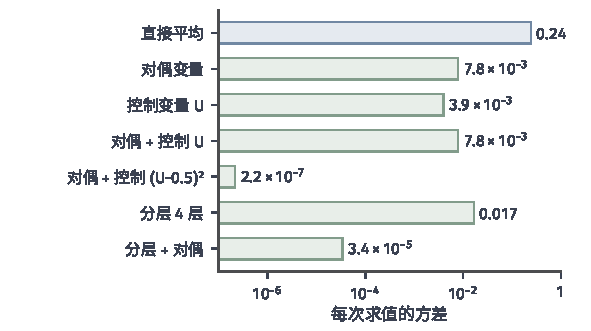
\includegraphics[width=100mm]{figures/07-probability/08-sampling-and-integration/matplotlib/budget-vr-combos/figure.pdf}
  \caption{计算$\mathbb{E}[\mathrm{e}^{U}]$时几种方差控制及其组合按每次求值折算的方差（数值积分精确计算，控制函数视为免费，控制系数取最优值）。蓝色为直接平均。“对偶 + 控制$U$”与单用对偶变量相同，因为配对后的控制量恒为$1/2$；控制函数改为对称的$(U-0.5)^{2}$后方差骤降。}
  \label{fig:budget-vr-combos}
\end{BookInlineFigure}

这组数字的教训是一般的：每种方法消去被积函数的某一部分波动，组合的效果取决于这些部分是否重叠。重叠时后一种方法无事可做，还白白付出成本；互补时效果可以远超任一方法单用。所以组合之后要按实际的估计量重新计算，第~\ref{chap:variance-reduction}章对单个方法证明的方差公式不能拼接使用。

\paragraph{高维均匀输入与变换后的函数}
拉丁超立方和随机化准蒙特卡洛作用在$[0,1)^{d}$的均匀输入上，被平均的是$F=f\circ T$，$T$是第~\ref{chap:sample-generation}章的生成映射。它们的改进依赖$F$的性质，而不是$f$的性质。拉丁超立方逐坐标均匀覆盖，对接近各坐标函数之和的$F$效果好，对主要由坐标间相互作用决定的$F$几乎无改进，有限样本下甚至可能不如独立抽样。随机化准蒙特卡洛的快速收敛要求$F$有一定的光滑性；若$T$是高斯的逆分布函数$\Phi^{-1}$，即使$f$光滑，$F$在立方体边界附近也无界，若$f$含示性函数，$F$在立方体内部有间断，两者都会使误差衰减变慢。选择这类方法时，要先检查变换后的函数，再按第~\ref{sec:budget-allocation}节选定$n$与$R$，误差只用组间方差估计。

\paragraph{两个方案的差}
比较两个方案的期望差$\mathbb{E}[A]-\mathbb{E}[B]$时，共同随机数用同一输入$U$生成$A(U)$与$B(U)$，由
\[
  \operatorname{Var}\bigl(A(U)-B(U)\bigr)=\operatorname{Var}(A)+\operatorname{Var}(B)-2\operatorname{Cov}\bigl(A(U),B(U)\bigr),
\]
正协方差越大，差的方差越小。与其他方法组合时要检查这种正协方差是否保留。若两个方案各自使用不同的重要性采样建议分布，同一个$U$在两边对应不同的样本位置，耦合可能失效；若两边都用逆变换且输出对输入单调同向，耦合通常最强。

用第~\ref{chap:variance-reduction}章的例子算一下：$A=\min\{X,1\}$，$X\sim\operatorname{Exp}(1)$；$B=\min\{Y,1\}$，$Y\sim\operatorname{Exp}(1.25)$；期望差约为$0.0613$。数值积分给出$\operatorname{Var}(A)\approx0.1289$、$\operatorname{Var}(B)\approx0.1291$。按差值的单对方差计，三种耦合方式的结果是
\[
  \underbrace{0.258}_{\text{独立输入}},\qquad\underbrace{0.0038}_{X,Y\text{用同一个}U},\qquad\underbrace{0.506}_{X\text{用}U,\ Y\text{用}1-U} .
\]
同向耦合把方差缩小约$68$倍；若误把对偶变量的反向配对用在差值上，协方差变负，方差反而比独立输入大近一倍。可见同一个“共用随机数”的操作，效果完全取决于两边输出对输入的单调方向。组合前后应各用一次小规模试运行，直接估计$\operatorname{Cov}(A,B)$，而不是假定它为正。

\subsection{梯度估计的选择}
\label{sec:budget-gradient-choice}

第~\ref{chap:expectation-gradient-estimation}章的三种表示分别依赖不同的条件。分布不随参数变化时，直接对被积函数求导；样本可写成$X=T_{\bm{\theta}}(\varepsilon)$且被积函数对样本位置可微时，用重参数化；能计算$\nabla_{\bm{\theta}}\ln p_{\bm{\theta}}$时，用得分函数，它不要求$f$对样本位置可微。离散样本空间上没有沿样本路径的导数，重参数化不能直接使用；状态数很少时还有一个更好的选择：直接求和。例如$X\sim\operatorname{Bern}(\theta)$时，$J(\theta)=\theta f(1)+(1-\theta)f(0)$，梯度$f(1)-f(0)$用两次求值就精确算出，没有任何随机误差。

条件都满足时，比较的依据仍是同一梯度任务下的偏差、方差与成本。不能预设重参数化总是方差更小，也不能预设得分函数总是更通用就更好。下面两个例子分别给出相反的结论。

\paragraph{被积函数振荡时}
设$X=\theta+\varepsilon$，$\varepsilon\sim\mathcal{N}(0,1)$，$f(x)=\sin(kx)$。由标准高斯的特征函数$\mathrm{e}^{-b^{2}/2}$，
\[
  J(\theta)=\sin(k\theta)\,\mathrm{e}^{-k^{2}/2},\qquad J'(\theta)=k\cos(k\theta)\,\mathrm{e}^{-k^{2}/2}.
\]
密度$\varphi(x-\theta)$的得分为$x-\theta$，在样本处等于$\varepsilon$，两种单样本估计分别是
\[
  \hat{g}_{\mathrm{R}}=k\cos\bigl(k(\theta+\varepsilon)\bigr),\qquad\hat{g}_{\mathrm{S}}=\sin\bigl(k(\theta+\varepsilon)\bigr)\,\varepsilon .
\]

用$\cos^{2}y=(1+\cos2y)/2$、$\sin^{2}y=(1-\cos2y)/2$及
\[
  \mathbb{E}\bigl[\cos(a+b\varepsilon)\bigr]=\cos a\,\mathrm{e}^{-b^{2}/2},\qquad\mathbb{E}\bigl[\varepsilon^{2}\cos(a+b\varepsilon)\bigr]=\cos a\,(1-b^{2})\,\mathrm{e}^{-b^{2}/2},
\]
两者的二阶矩分别为
\[
  \frac{k^{2}}{2}\bigl(1+\cos(2k\theta)\,\mathrm{e}^{-2k^{2}}\bigr),\qquad\frac12-\frac12\cos(2k\theta)\,(1-4k^{2})\,\mathrm{e}^{-2k^{2}} .
\]
减去梯度的平方即得方差。$k$较大时重参数化的方差约为$k^{2}/2$，得分函数的方差约为$1/2$：重参数化把$f$的导数带进估计，振荡越快，导数的幅度越大；得分函数只用到$f$的值，而$\lvert\sin\rvert\le1$。

图~\ref{fig:budget-gradient-variance}(a)取$\theta=0.3$，两条曲线在$k\approx1.09$相交。$k=0.5$时重参数化的方差约$0.0071$，得分函数约$0.31$，前者好四十多倍；$k=3$时前者约$4.50$，后者约$0.50$，后者好九倍。重参数化还要计算$f'$，每个样本的成本通常更高，所以$k$较大时得分函数在工作量归一化方差上的优势更明显。$2\times10^{6}$个样本的模拟（种子$1$）在$k=1$与$k=3$处与上面的公式相差不到$1\%$。

\begin{BookInlineFigure}
  \centering
  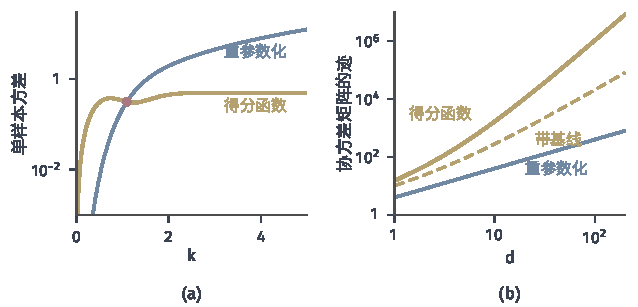
\includegraphics[width=108mm]{figures/07-probability/08-sampling-and-integration/matplotlib/budget-gradient-variance/figure.pdf}
  \caption{同一梯度任务下两种估计的单样本方差。(a)~$J(\theta)=\mathbb{E}[\sin(kX)]$，$X\sim\mathcal{N}(\theta,1)$，$\theta=0.3$：蓝线为重参数化，黄线为得分函数，红点为交点$k\approx1.09$。(b)~$J(\bm{\theta})=\mathbb{E}\lVert\bm{X}\rVert_2^{2}$，$\bm{X}\sim\mathcal{N}(\bm{\theta},\bm{I}_d)$，$\bm{\theta}=\bm{0}$：协方差矩阵的迹随维数$d$的变化，黄色虚线为得分函数减去基线$d$之后。}
  \label{fig:budget-gradient-variance}
\end{BookInlineFigure}

\paragraph{维数增大时}
设$\bm{X}=\bm{\theta}+\bm{\varepsilon}$，$\bm{\varepsilon}\sim\mathcal{N}(\bm{0},\bm{I}_d)$，$f(\bm{x})=\lVert\bm{x}\rVert_2^{2}$，在$\bm{\theta}=\bm{0}$处求梯度，真值为$\bm{0}$。

重参数化的估计是$2\bm{X}$，协方差矩阵为$4\bm{I}_d$，迹为$4d$。得分函数的估计是$\lVert\bm{X}\rVert_2^{2}\bm{X}$，由于真值为零，迹等于二阶矩$\mathbb{E}\lVert\bm{\varepsilon}\rVert_2^{6}$。$S=\lVert\bm{\varepsilon}\rVert_2^{2}$服从$\chi^{2}_{d}$，其各阶矩为
\[
  \mathbb{E}[S]=d,\qquad\mathbb{E}[S^{2}]=d(d+2),\qquad\mathbb{E}[S^{3}]=d(d+2)(d+4),
\]
于是
\[
  \operatorname{tr}\bm{\Sigma}_{\text{得分}}=\mathbb{E}\lVert\bm{\varepsilon}\rVert_2^{6}=d(d+2)(d+4).
\]
减去与样本独立的基线$b=\mathbb{E}\lVert\bm{X}\rVert_2^{2}=d$后，估计变为$(\lVert\bm{X}\rVert_2^{2}-d)\bm{X}$，其迹为
\[
  \begin{aligned}
    \mathbb{E}\bigl[(S-d)^{2}S\bigr]&=\mathbb{E}[S^{3}]-2d\,\mathbb{E}[S^{2}]+d^{2}\,\mathbb{E}[S]\\
    &=d(d+2)(d+4)-2d^{2}(d+2)+d^{3}=2d^{2}+8d .
  \end{aligned}
\]
基线把三次增长降成二次，但仍比重参数化的$4d$大约$d/2$倍。图~\ref{fig:budget-gradient-variance}(b)在对数坐标上显示了这三条曲线：$d=100$时分别为$400$、约$1.06\times10^{6}$与$20\,800$。这里重参数化每个样本要计算一次$\nabla f$，用反向自动求导时其成本是$f$的常数倍，与$d$无关，抵消不了$d/2$倍的方差差距。

\paragraph{可微性的条件}
重参数化的前提是把求导与求期望交换。$f$不连续时这一步可能失败而不报错。取$f(x)=\mathbf{1}_{\{x>0\}}$，$X=\theta+\varepsilon$，则$J(\theta)=\Phi(\theta)$，梯度为$\varphi(\theta)>0$；但对几乎每个$\varepsilon$，$\mathbf{1}_{\{\theta+\varepsilon>0\}}$在$\theta$附近是常数，路径导数为零，重参数化的估计恒为$0$。得分函数的估计$\mathbf{1}_{\{X>0\}}(X-\theta)$在这里无偏。所以选择重参数化之前，要先按第~\ref{chap:expectation-gradient-estimation}章检查交换条件，而不是看程序能否算出导数。

综合起来，梯度估计的选择依次回答四个问题：分布是否随参数变化；样本空间是否离散且小到可以直接求和；能否沿生成映射求导，且交换条件成立；能否计算得分。满足条件的估计都列出后，按式~\eqref{eq:budget-vector-mse}的迹或所需方向上的方差，乘以每个样本的成本来比较。参数怎样依据这些梯度更新，可参考\BookChapterRef{chap:stochastic-gradient-methods}{卷五第13章“随机梯度方法”}，那里梯度估计的方差直接影响步长的选择与收敛速度。
